\chapter{Results}
\label{sec:results}

\section{Charging without photoemission}

\section{Charging with photoemission}

\subsection*{Drift parallel to X axis}

\begin{center}
    \begin{figure}[H]
      \begin{subfigure}[b]{0.61\textwidth}
      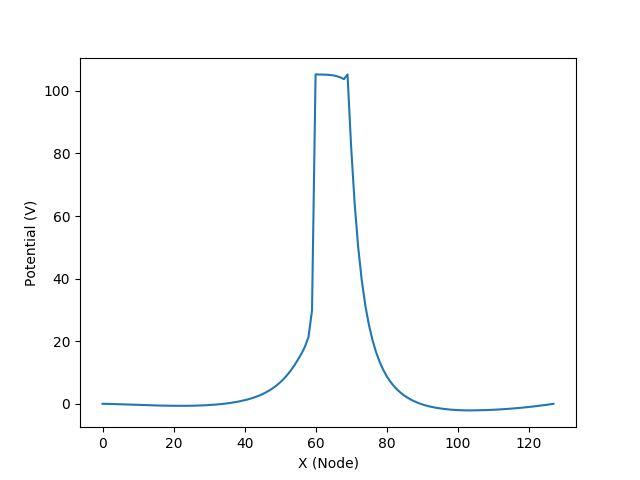
\includegraphics[width=\textwidth]{figures/MMO/plusX/Booms/PhiXBoomsPlusX.png}
      \caption{Booms}
      \label{fig:PhiXBoomsPlusX}
    \end{subfigure}
    \begin{subfigure}[b]{0.61\textwidth}
      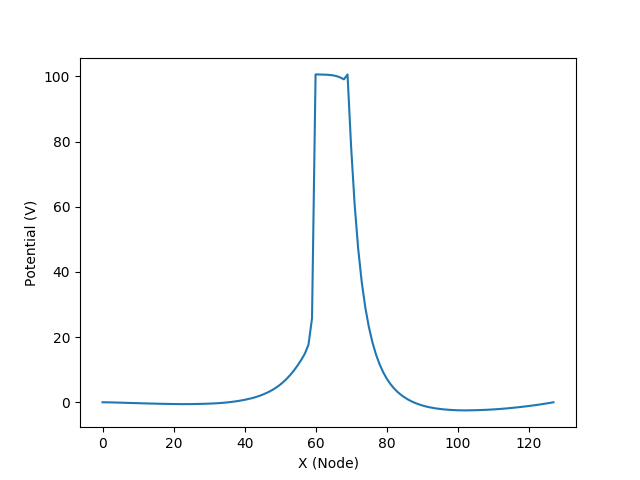
\includegraphics[width=\textwidth]{figures/MMO/plusX/noBooms/PhiXnoBoomsPlusX.png}
      \caption{Without booms}
      \label{fig:PhiXnoBoomsPlusX}
    \end{subfigure}
  \label{fig:PhiXDriftX}
  \caption{Dummy text}
  \end{figure}
\end{center}

\begin{center}
\begin{figure}[H]
  \begin{subfigure}[b]{0.61\textwidth}
    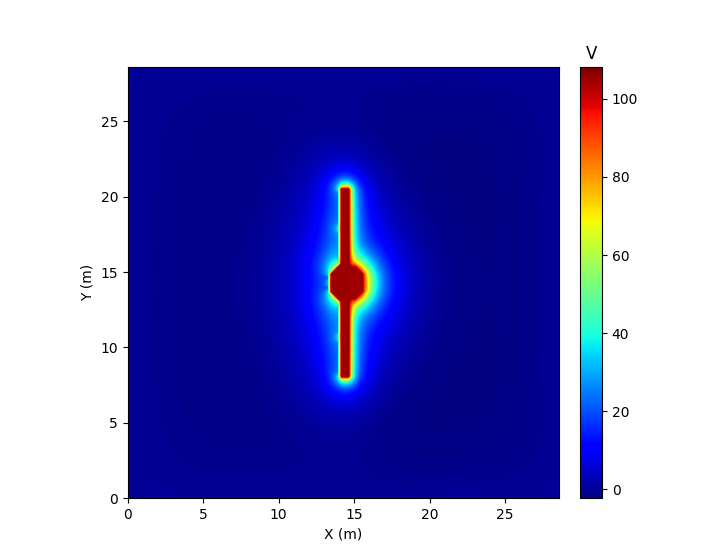
\includegraphics[width=\textwidth]{figures/MMO/plusX/Booms/AvgAfter1000BoomsPlusX.png}
    \caption{Booms}
    \label{fig:AvgAfter1000BoomsPlusX}
  \end{subfigure}
  \hfill
  \begin{subfigure}[b]{0.61\textwidth}
    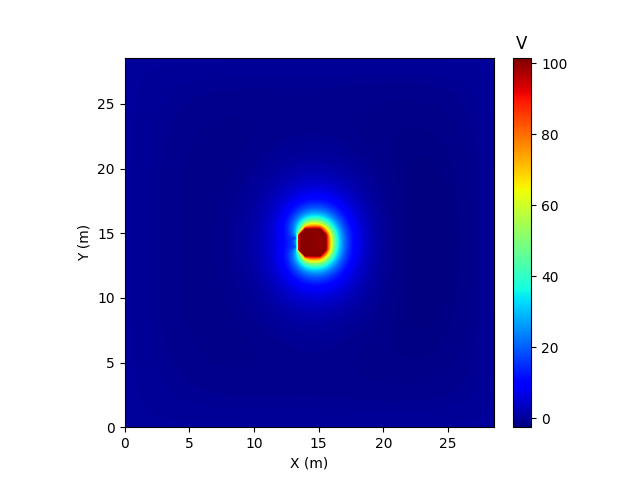
\includegraphics[width=\textwidth]{figures/MMO/plusX/noBooms/AvgAfter1000noBoomsPlusX.png}
    \caption{Without booms}
    \label{fig:AvgAfter1000noBoomsPlusX}
  \end{subfigure}
  \label{fig:AvgPhiDriftX}
  \caption{Dummy text}
\end{figure}
\end{center}



\subsection*{Drift parallel to Z axis}


\section{Charging in an external magnetic field}

\section{Charging at different photoelectron temperatures}